%%==================================================
%% chapter03.tex for SJTU Master Thesis
%% Encoding: UTF-8
%%==================================================

\chapter{混合现实眼镜下的三维界面设计}
\label{chap:3DUI}

本章将介绍本文所设计的混合现实眼镜交互系统的第一个部分:三维界面。
三维界面的想法来源于增强现实应用中用户所触及到的三维事物。
大家已经熟悉的桌面应用界面为WIMP系列,二维的界面对应二维的输入,而现在手机、平板上的界面也开始随着设备慢慢地变化,由此本文所设计的系统根据整个操控环境都是三维的前提专门设计了一套三维界面。首先介绍适合增强现实交互界面的设计原则,接着呈现效果,这套三维交互界面将应用在第\ref{chap:interaction}章的交互研究中。

\section{设计原则}

基于\ref{sec:related-cur}节调研的研究现状,本节首先总结出适合增强现实交互界面的设计原则。
该原则主要为避免对识别准确性的影响,减少用户的记忆负担,同时增强交互的用户体验,列举如下:

\label{sec:design-principle}
\begin{enumerate}
\item 不在手上佩戴笨重的设备

由\ref{sec:related-jiaohu}节提到的相关工作可以看到不少精心制作的增强现实设备,然而若是佩戴复杂或者笨重的设备在手上会导致两个问题。
其一,用户体验下降,除了交互之外用户还会被设备的触感,重量等干扰,无法更自如地进行交互;
其二,用户极有可能在使用过程中对设备造成人为影响,比如无意中影响了预设的配置环境,旋转了uTrack\upcite{uTrack}
上的传感器,就会影响输入检测的正确性。
因此从舒适性和正确性角度出发,本文系统的设备将尽量减少手上复杂或笨重的设备佩戴。

\item 保持交互的一致性

试想如果一个增强现实应用中的操控和物理世界有着对应,却用着截然不同的交互手段,则势必会影响用
户在操控时的感受,并且增加记忆的复杂度。所以尽量保留物理世界的交互方式有助于用户尽快适应系统。
同时在物理世界无法做到的功能上,体现增强现实交互的优势,比如用户无法碰触远方的物体因而无法操控,但在增强现实应用环境下就可以实现这一点,
本文工作在对交互一致性的保持上进行改进的设计。

\item 尽可能少的手势设计

这一点同样是出于帮助用户快速适应改进后系统的考虑。
如果一个系统的手势指令太多,用户的记忆复杂度就会增加,可能需要进行一定时间的训练或者每次
都要仔细回顾一番才能再一次适应该系统。
为了让用户迅速学会使用该系统且经久不忘,本文系统最终只设计了三个手势,将在第\ref{chap:interaction}章中详述。

\item 明显的状态切换

在\ref{sec:related-zhuangtai}节中提到通过遮盖两个图案来进行状
态切换的系统\upcite{TrackingBased}。
在实验中,用户经常忘记遮盖指定图案来发送指令,也就是由于状态切换的指令不够明显和
简单,给使用者增加了难度,导致用户的错误指令,
故而系统将设计简单明了的状态切换方式,提升易用性。

\end{enumerate}

根据以上原则,本文设计了手掌召唤式菜单、目标跟踪式菜单和屏幕固定式这三种菜单,具体阐述如下。

%\section{设计结果展示}

\section{手掌召唤式菜单}
\label{sec:palm-based}
\begin{figure}[!htp]
  \centering
  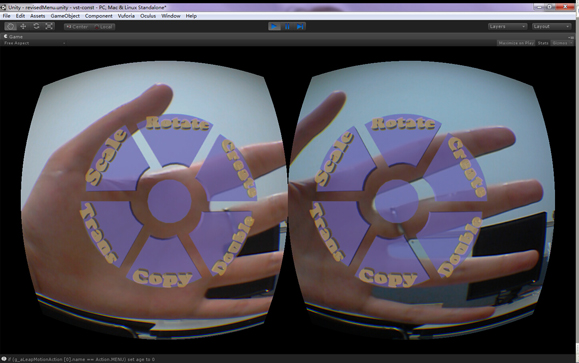
\includegraphics[width=0.8\textwidth]{chap3/palm-basedMenu}
  \bicaption[fig:palm-based]{手掌召唤式菜单}{手掌召唤式菜单}{Fig.}{Palm-based menus}
\end{figure}

手掌召唤式菜单是用户通过手掌手势召唤而
成的菜单,顾名思义位置始终固定在手掌上。为了让菜单和用户
更加融合,本文所设计的系统依据手掌的形状,借鉴调色盘的
概念设计出了该菜单,也是区别于以往直接将二维菜单或者基本图元照搬的一个特点。
用户通过拣选菜单上不同的
指令,然后选中物体对其进行相应的操作,就如同
将调色盘上不同的颜色分配在不同的物体上一样。
如图\ref{fig:palm-based}所示,当摄像头捕获到菜单指令后,在用户手掌正中心出现的就是该菜单,就像是用户手握的一个道具一样。

手掌召唤式菜单含有以下几个选项:创建物体、单手移动物体、单手旋转物体、单手放缩物体、双手操控物体和拷贝物体。
操控类菜单选中后需要指定目标物,可以一个,可以多个。
用户单手操控物体时需要选择不同指令进行不同操作,而用户双手操控物体时,只需要选择双手操控物体的命令即可。
随后系统将根据用户双手间的相对移动,以时间为轴判断用户在进行平移放缩还是旋转。

\section{目标跟踪式菜单}
\begin{figure}[!htp]
  \centering
  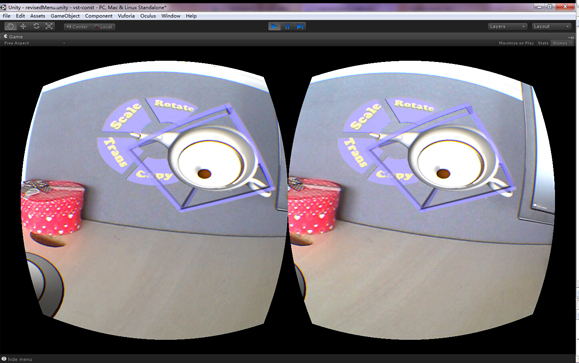
\includegraphics[width=0.8\textwidth]{chap3/object-trackedMenu}
  \bicaption[fig:object-tracked]{目标跟踪式菜单}{目标跟踪式菜单}{Fig.}{object-tracked menus}
\end{figure}

目标跟踪式和手掌召唤式菜单触发方式属于两种类型,后者通过用户的手召唤出来,是基于操作的一种菜单调用;
而前者则是通过选中场景内已经存在的物体,目标跟踪式菜单会出现在该物体周围,随物体的位置变化而变化,选择具体的指令后,该指令就会作用在被选中的物体上,属于基于目标物的一种菜单调用。
如图\ref{fig:object-tracked}所示,召唤出的菜单卡在被选中目标物的一侧。

目标跟踪式菜单有以下几个选项:单手移动物体,单手旋转物体,单手放缩物体,双手操控物体和拷贝物体。和\ref{sec:palm-based}节的功能描述类似。
在操作顺序上由于已经选中物体,于是选完菜单后就可以直接进行操控。

\section{屏幕固定式菜单}
\begin{figure}[!htp]
  \centering
  \subfigure{\label{fig:screen-fixed:1}}\addtocounter{subfigure}{-2}
	\subfigure[Screen-fixed menus sample one]{\subfigure[屏幕固定式菜单示例一]
		{\includegraphics[width=0.4\textwidth]{chap3/screen-fixedMenu1}}}
	\subfigure{\label{fig:screen-fixed:2}}\addtocounter{subfigure}{-2}
	\subfigure[Screen-fixed menus sample two]{\subfigure[屏幕固定式菜单示例二]
		{\includegraphics[width=0.4\textwidth]{chap3/screen-fixedMenu2}}}
  \bicaption[fig:screen-fixed]{屏幕固定式菜单}{屏幕固定式菜单}{Fig.}{Screen-fixed menus}
\end{figure}

屏幕固定式菜单和目标跟踪式菜单的触发方式相同,都属于基于目标物的菜单调用,但选中物体后,屏幕固定式菜单会固定在屏幕正中央,无论选中的物体在哪里,用户如何改变视角,该菜单都会出现在相同的位置,大小和角度都不会变化。
如图\ref{fig:screen-fixed}(a)所示,当选中了茶壶后,茶壶附近出现选中立体框,并在屏幕正中央出现菜单,
而后佩戴ARGlasses的用户向左转头如图\ref{fig:screen-fixed}(b)所示,整个场景变动,茶壶不在视野范围内,但该菜单依然固定在屏幕正中央。

以上三种菜单中,手掌召唤式菜单属于基于操作的菜单类型,选择统一的菜单指令后,可以将指令附着到多个物体上。
而目标跟踪式菜单与屏幕固定式菜单从单个物体出发,偏向个性化操作。
三种菜单在混合现实眼镜下的效果会在第\ref{chap:exp}章详细评估。

\section{三种布局的菜单对照与分析}

\begin{table}[!hpbt]\renewcommand{\arraystretch}{1.1}
  \centering
  \bicaption[table:3dmenu]{本文工作所设计的三种菜单对比}{本文工作所设计的三种菜单对比}{Table}{Comparison among three styles of 3D menus in this work}
\begin{tabular}{*{4}{L{.23\textwidth}}} \toprule
    分析内容 & 手掌召唤式菜单 & 目标跟踪式菜单 & 屏幕固定式菜单 \\
	\midrule
    特点描述 	&
	随手掌召唤而出,位置随手变化 		&
 	由选中物体触发,位置随物体变化 &
	%\vspace{1em}
	\hspace{100pt}由选中物体触发,位置固定在屏幕正中央\\	
	%\vspace{0.5em}
	设计原则一:\hspace{15pt}不在手上佩戴笨重的设备 &
	无任何佩戴物 &
	需佩戴色环选中物体 &
	需佩戴色环选中物体 &\\
%	\vspace{0.8em}
	设计原则二:\hspace{15pt}保持交互的一致性 &
	额外设计手掌触发菜单 &
	选中物体出菜单,与二维菜单习惯一致 &
	选中物体出菜单,与二维菜单习惯一致 &\\
%	\vspace{1em}
	设计原则三:\hspace{15pt}尽可能少的手势设计&
	新增手掌手势&
	选择手势与日常选中手势相似&
	选择手势与日常选中手势相似&\\
%	\vspace{0.3em}
	设计原则四:\hspace{15pt}明显的状态切换&
	通过手掌识别菜单模式&
	通过色环分离控制与选择指令&
	通过色环分离控制与选择指令&
	\bottomrule
  \end{tabular}
\end{table}

由表\ref{table:3dmenu}可见本文设计的三种布局的菜单。手掌召唤式菜单随手掌召唤而出,然后指定物体,是操作先于目标的一种思考方式,
目标跟踪式菜单指定物体然后显示,和屏幕固定式菜单相同,是目标先于操作的一种思考方式。
而这二者的区别在于菜单的位置,前者随目标物移动,而后者固定在屏幕中央。
前者的设计思路将菜单作为目标物的一种属性,将菜单镶嵌在目标物周围;
后者从更直观的显示角度出发。
在设计原则的应用上,三者都尽量减少了额外的佩戴物,即便是色环也是轻量级的物体;
手掌召唤式菜单额外增加了手掌召唤菜单的交互,但并没有和现实生活中的交互产生矛盾,对用户产生的记忆压力也不大,另两者没有新增交互和手势设计;
最后手掌手势和色环成功分离了自己的状态和其他状态,做到了明显的状态切换这一原则。

\section{本章小结}
本章主要介绍了本文所设计的系统使用的三维界面。
首先通过对相关工作的理解提出了设计原则,设计原则应用于三维界面设计。
然后列举了设计的三种菜单。
手掌召唤式菜单以操作为重点,先选菜单再选目标物,并且手掌召唤式菜单卡位于掌心,将用户的手变成了一个增强现实界面。
目标跟踪式菜单和屏幕固定式菜单均以目标物为重点,先选择想要操作的物体,然后再选择想要实行的功能。
并且采用了两种风格的布局,目标跟踪式菜单会随目标物而移动,屏幕固定式菜单则始终固定在屏幕正中央,无论用户看向何方都能看到嵌在屏幕中央的菜单,便于选择。
除此之外介绍了本文系统设计的几个菜单,分别是创建、单手操控菜单组、双手操控和拷贝物体。
对菜单进一步的评估将在第\ref{chap:exp}章展开。